% GNUPLOT: LaTeX picture with Postscript
\begingroup
  \makeatletter
  \providecommand\color[2][]{%
    \GenericError{(gnuplot) \space\space\space\@spaces}{%
      Package color not loaded in conjunction with
      terminal option `colourtext'%
    }{See the gnuplot documentation for explanation.%
    }{Either use 'blacktext' in gnuplot or load the package
      color.sty in LaTeX.}%
    \renewcommand\color[2][]{}%
  }%
  \providecommand\includegraphics[2][]{%
    \GenericError{(gnuplot) \space\space\space\@spaces}{%
      Package graphicx or graphics not loaded%
    }{See the gnuplot documentation for explanation.%
    }{The gnuplot epslatex terminal needs graphicx.sty or graphics.sty.}%
    \renewcommand\includegraphics[2][]{}%
  }%
  \providecommand\rotatebox[2]{#2}%
  \@ifundefined{ifGPcolor}{%
    \newif\ifGPcolor
    \GPcolortrue
  }{}%
  \@ifundefined{ifGPblacktext}{%
    \newif\ifGPblacktext
    \GPblacktexttrue
  }{}%
  % define a \g@addto@macro without @ in the name:
  \let\gplgaddtomacro\g@addto@macro
  % define empty templates for all commands taking text:
  \gdef\gplbacktext{}%
  \gdef\gplfronttext{}%
  \makeatother
  \ifGPblacktext
    % no textcolor at all
    \def\colorrgb#1{}%
    \def\colorgray#1{}%
  \else
    % gray or color?
    \ifGPcolor
      \def\colorrgb#1{\color[rgb]{#1}}%
      \def\colorgray#1{\color[gray]{#1}}%
      \expandafter\def\csname LTw\endcsname{\color{white}}%
      \expandafter\def\csname LTb\endcsname{\color{black}}%
      \expandafter\def\csname LTa\endcsname{\color{black}}%
      \expandafter\def\csname LT0\endcsname{\color[rgb]{1,0,0}}%
      \expandafter\def\csname LT1\endcsname{\color[rgb]{0,1,0}}%
      \expandafter\def\csname LT2\endcsname{\color[rgb]{0,0,1}}%
      \expandafter\def\csname LT3\endcsname{\color[rgb]{1,0,1}}%
      \expandafter\def\csname LT4\endcsname{\color[rgb]{0,1,1}}%
      \expandafter\def\csname LT5\endcsname{\color[rgb]{1,1,0}}%
      \expandafter\def\csname LT6\endcsname{\color[rgb]{0,0,0}}%
      \expandafter\def\csname LT7\endcsname{\color[rgb]{1,0.3,0}}%
      \expandafter\def\csname LT8\endcsname{\color[rgb]{0.5,0.5,0.5}}%
    \else
      % gray
      \def\colorrgb#1{\color{black}}%
      \def\colorgray#1{\color[gray]{#1}}%
      \expandafter\def\csname LTw\endcsname{\color{white}}%
      \expandafter\def\csname LTb\endcsname{\color{black}}%
      \expandafter\def\csname LTa\endcsname{\color{black}}%
      \expandafter\def\csname LT0\endcsname{\color{black}}%
      \expandafter\def\csname LT1\endcsname{\color{black}}%
      \expandafter\def\csname LT2\endcsname{\color{black}}%
      \expandafter\def\csname LT3\endcsname{\color{black}}%
      \expandafter\def\csname LT4\endcsname{\color{black}}%
      \expandafter\def\csname LT5\endcsname{\color{black}}%
      \expandafter\def\csname LT6\endcsname{\color{black}}%
      \expandafter\def\csname LT7\endcsname{\color{black}}%
      \expandafter\def\csname LT8\endcsname{\color{black}}%
    \fi
  \fi
    \setlength{\unitlength}{0.0500bp}%
    \ifx\gptboxheight\undefined%
      \newlength{\gptboxheight}%
      \newlength{\gptboxwidth}%
      \newsavebox{\gptboxtext}%
    \fi%
    \setlength{\fboxrule}{0.5pt}%
    \setlength{\fboxsep}{1pt}%
\begin{picture}(9620.00,9620.00)%
    \gplgaddtomacro\gplbacktext{%
      \csname LTb\endcsname%
      \put(966,6624){\makebox(0,0)[r]{\strut{}$10^{-3}$}}%
      \csname LTb\endcsname%
      \put(966,7022){\makebox(0,0)[r]{\strut{}$10^{-2}$}}%
      \csname LTb\endcsname%
      \put(966,7419){\makebox(0,0)[r]{\strut{}$10^{-1}$}}%
      \csname LTb\endcsname%
      \put(966,7817){\makebox(0,0)[r]{\strut{}$10^{0}$}}%
      \csname LTb\endcsname%
      \put(966,8215){\makebox(0,0)[r]{\strut{}$10^{1}$}}%
      \csname LTb\endcsname%
      \put(966,8613){\makebox(0,0)[r]{\strut{}$10^{2}$}}%
      \csname LTb\endcsname%
      \put(966,9010){\makebox(0,0)[r]{\strut{}$10^{3}$}}%
      \csname LTb\endcsname%
      \put(966,9408){\makebox(0,0)[r]{\strut{}$10^{4}$}}%
      \csname LTb\endcsname%
      \put(1068,6445){\makebox(0,0){\strut{} }}%
      \csname LTb\endcsname%
      \put(1427,6445){\makebox(0,0){\strut{} }}%
      \csname LTb\endcsname%
      \put(1786,6445){\makebox(0,0){\strut{} }}%
      \csname LTb\endcsname%
      \put(2145,6445){\makebox(0,0){\strut{} }}%
      \csname LTb\endcsname%
      \put(2504,6445){\makebox(0,0){\strut{} }}%
      \csname LTb\endcsname%
      \put(2863,6445){\makebox(0,0){\strut{} }}%
      \csname LTb\endcsname%
      \put(3223,6445){\makebox(0,0){\strut{} }}%
      \csname LTb\endcsname%
      \put(3582,6445){\makebox(0,0){\strut{} }}%
      \csname LTb\endcsname%
      \put(3941,6445){\makebox(0,0){\strut{} }}%
      \csname LTb\endcsname%
      \put(4300,6445){\makebox(0,0){\strut{} }}%
      \csname LTb\endcsname%
      \put(4659,6445){\makebox(0,0){\strut{} }}%
      \csname LTb\endcsname%
      \put(4761,6624){\makebox(0,0)[l]{\strut{} }}%
      \csname LTb\endcsname%
      \put(4761,6902){\makebox(0,0)[l]{\strut{} }}%
      \csname LTb\endcsname%
      \put(4761,7181){\makebox(0,0)[l]{\strut{} }}%
      \csname LTb\endcsname%
      \put(4761,7459){\makebox(0,0)[l]{\strut{} }}%
      \csname LTb\endcsname%
      \put(4761,7738){\makebox(0,0)[l]{\strut{} }}%
      \csname LTb\endcsname%
      \put(4761,8016){\makebox(0,0)[l]{\strut{} }}%
      \csname LTb\endcsname%
      \put(4761,8294){\makebox(0,0)[l]{\strut{} }}%
      \csname LTb\endcsname%
      \put(4761,8573){\makebox(0,0)[l]{\strut{} }}%
      \csname LTb\endcsname%
      \put(4761,8851){\makebox(0,0)[l]{\strut{} }}%
      \csname LTb\endcsname%
      \put(4761,9130){\makebox(0,0)[l]{\strut{} }}%
      \csname LTb\endcsname%
      \put(4761,9408){\makebox(0,0)[l]{\strut{} }}%
      \csname LTb\endcsname%
      \put(1068,9587){\makebox(0,0){\strut{}$10^{2}$}}%
      \csname LTb\endcsname%
      \put(1786,9587){\makebox(0,0){\strut{}$10^{3}$}}%
      \csname LTb\endcsname%
      \put(2504,9587){\makebox(0,0){\strut{}$10^{4}$}}%
      \csname LTb\endcsname%
      \put(3223,9587){\makebox(0,0){\strut{}$10^{5}$}}%
      \csname LTb\endcsname%
      \put(3941,9587){\makebox(0,0){\strut{}$10^{6}$}}%
      \csname LTb\endcsname%
      \put(4659,9587){\makebox(0,0){\strut{}$10^{7}$}}%
    }%
    \gplgaddtomacro\gplfronttext{%
      \csname LTb\endcsname%
      \put(366,8016){\rotatebox{-270}{\makebox(0,0){\strut{}$k = 2$}}}%
    }%
    \gplgaddtomacro\gplbacktext{%
      \csname LTb\endcsname%
      \put(4858,6624){\makebox(0,0)[r]{\strut{} }}%
      \csname LTb\endcsname%
      \put(4858,6902){\makebox(0,0)[r]{\strut{} }}%
      \csname LTb\endcsname%
      \put(4858,7181){\makebox(0,0)[r]{\strut{} }}%
      \csname LTb\endcsname%
      \put(4858,7459){\makebox(0,0)[r]{\strut{} }}%
      \csname LTb\endcsname%
      \put(4858,7738){\makebox(0,0)[r]{\strut{} }}%
      \csname LTb\endcsname%
      \put(4858,8016){\makebox(0,0)[r]{\strut{} }}%
      \csname LTb\endcsname%
      \put(4858,8294){\makebox(0,0)[r]{\strut{} }}%
      \csname LTb\endcsname%
      \put(4858,8573){\makebox(0,0)[r]{\strut{} }}%
      \csname LTb\endcsname%
      \put(4858,8851){\makebox(0,0)[r]{\strut{} }}%
      \csname LTb\endcsname%
      \put(4858,9130){\makebox(0,0)[r]{\strut{} }}%
      \csname LTb\endcsname%
      \put(4858,9408){\makebox(0,0)[r]{\strut{} }}%
      \csname LTb\endcsname%
      \put(4960,6445){\makebox(0,0){\strut{} }}%
      \csname LTb\endcsname%
      \put(5319,6445){\makebox(0,0){\strut{} }}%
      \csname LTb\endcsname%
      \put(5678,6445){\makebox(0,0){\strut{} }}%
      \csname LTb\endcsname%
      \put(6037,6445){\makebox(0,0){\strut{} }}%
      \csname LTb\endcsname%
      \put(6396,6445){\makebox(0,0){\strut{} }}%
      \csname LTb\endcsname%
      \put(6755,6445){\makebox(0,0){\strut{} }}%
      \csname LTb\endcsname%
      \put(7114,6445){\makebox(0,0){\strut{} }}%
      \csname LTb\endcsname%
      \put(7473,6445){\makebox(0,0){\strut{} }}%
      \csname LTb\endcsname%
      \put(7832,6445){\makebox(0,0){\strut{} }}%
      \csname LTb\endcsname%
      \put(8191,6445){\makebox(0,0){\strut{} }}%
      \csname LTb\endcsname%
      \put(8550,6445){\makebox(0,0){\strut{} }}%
      \csname LTb\endcsname%
      \put(8652,6624){\makebox(0,0)[l]{\strut{}$10^{-3}$}}%
      \csname LTb\endcsname%
      \put(8652,7022){\makebox(0,0)[l]{\strut{}$10^{-2}$}}%
      \csname LTb\endcsname%
      \put(8652,7419){\makebox(0,0)[l]{\strut{}$10^{-1}$}}%
      \csname LTb\endcsname%
      \put(8652,7817){\makebox(0,0)[l]{\strut{}$10^{0}$}}%
      \csname LTb\endcsname%
      \put(8652,8215){\makebox(0,0)[l]{\strut{}$10^{1}$}}%
      \csname LTb\endcsname%
      \put(8652,8613){\makebox(0,0)[l]{\strut{}$10^{2}$}}%
      \csname LTb\endcsname%
      \put(8652,9010){\makebox(0,0)[l]{\strut{}$10^{3}$}}%
      \csname LTb\endcsname%
      \put(8652,9408){\makebox(0,0)[l]{\strut{}$10^{4}$}}%
      \csname LTb\endcsname%
      \put(4960,9587){\makebox(0,0){\strut{}$10^{2}$}}%
      \csname LTb\endcsname%
      \put(5678,9587){\makebox(0,0){\strut{}$10^{3}$}}%
      \csname LTb\endcsname%
      \put(6396,9587){\makebox(0,0){\strut{}$10^{4}$}}%
      \csname LTb\endcsname%
      \put(7114,9587){\makebox(0,0){\strut{}$10^{5}$}}%
      \csname LTb\endcsname%
      \put(7832,9587){\makebox(0,0){\strut{}$10^{6}$}}%
      \csname LTb\endcsname%
      \put(8550,9587){\makebox(0,0){\strut{}$10^{7}$}}%
    }%
    \gplgaddtomacro\gplfronttext{%
      \csname LTb\endcsname%
      \put(9250,8016){\rotatebox{-270}{\makebox(0,0){\strut{}$k = 3$}}}%
    }%
    \gplgaddtomacro\gplbacktext{%
      \csname LTb\endcsname%
      \put(966,3417){\makebox(0,0)[r]{\strut{}$10^{-3}$}}%
      \csname LTb\endcsname%
      \put(966,3815){\makebox(0,0)[r]{\strut{}$10^{-2}$}}%
      \csname LTb\endcsname%
      \put(966,4213){\makebox(0,0)[r]{\strut{}$10^{-1}$}}%
      \csname LTb\endcsname%
      \put(966,4611){\makebox(0,0)[r]{\strut{}$10^{0}$}}%
      \csname LTb\endcsname%
      \put(966,5008){\makebox(0,0)[r]{\strut{}$10^{1}$}}%
      \csname LTb\endcsname%
      \put(966,5406){\makebox(0,0)[r]{\strut{}$10^{2}$}}%
      \csname LTb\endcsname%
      \put(966,5804){\makebox(0,0)[r]{\strut{}$10^{3}$}}%
      \csname LTb\endcsname%
      \put(966,6202){\makebox(0,0)[r]{\strut{}$10^{4}$}}%
      \csname LTb\endcsname%
      \put(1068,3238){\makebox(0,0){\strut{} }}%
      \csname LTb\endcsname%
      \put(1786,3238){\makebox(0,0){\strut{} }}%
      \csname LTb\endcsname%
      \put(2504,3238){\makebox(0,0){\strut{} }}%
      \csname LTb\endcsname%
      \put(3223,3238){\makebox(0,0){\strut{} }}%
      \csname LTb\endcsname%
      \put(3941,3238){\makebox(0,0){\strut{} }}%
      \csname LTb\endcsname%
      \put(4659,3238){\makebox(0,0){\strut{} }}%
      \csname LTb\endcsname%
      \put(4761,3417){\makebox(0,0)[l]{\strut{} }}%
      \csname LTb\endcsname%
      \put(4761,3695){\makebox(0,0)[l]{\strut{} }}%
      \csname LTb\endcsname%
      \put(4761,3974){\makebox(0,0)[l]{\strut{} }}%
      \csname LTb\endcsname%
      \put(4761,4252){\makebox(0,0)[l]{\strut{} }}%
      \csname LTb\endcsname%
      \put(4761,4531){\makebox(0,0)[l]{\strut{} }}%
      \csname LTb\endcsname%
      \put(4761,4809){\makebox(0,0)[l]{\strut{} }}%
      \csname LTb\endcsname%
      \put(4761,5088){\makebox(0,0)[l]{\strut{} }}%
      \csname LTb\endcsname%
      \put(4761,5366){\makebox(0,0)[l]{\strut{} }}%
      \csname LTb\endcsname%
      \put(4761,5645){\makebox(0,0)[l]{\strut{} }}%
      \csname LTb\endcsname%
      \put(4761,5923){\makebox(0,0)[l]{\strut{} }}%
      \csname LTb\endcsname%
      \put(4761,6202){\makebox(0,0)[l]{\strut{} }}%
      \csname LTb\endcsname%
      \put(1068,6381){\makebox(0,0){\strut{} }}%
      \csname LTb\endcsname%
      \put(1427,6381){\makebox(0,0){\strut{} }}%
      \csname LTb\endcsname%
      \put(1786,6381){\makebox(0,0){\strut{} }}%
      \csname LTb\endcsname%
      \put(2145,6381){\makebox(0,0){\strut{} }}%
      \csname LTb\endcsname%
      \put(2504,6381){\makebox(0,0){\strut{} }}%
      \csname LTb\endcsname%
      \put(2863,6381){\makebox(0,0){\strut{} }}%
      \csname LTb\endcsname%
      \put(3223,6381){\makebox(0,0){\strut{} }}%
      \csname LTb\endcsname%
      \put(3582,6381){\makebox(0,0){\strut{} }}%
      \csname LTb\endcsname%
      \put(3941,6381){\makebox(0,0){\strut{} }}%
      \csname LTb\endcsname%
      \put(4300,6381){\makebox(0,0){\strut{} }}%
      \csname LTb\endcsname%
      \put(4659,6381){\makebox(0,0){\strut{} }}%
    }%
    \gplgaddtomacro\gplfronttext{%
      \csname LTb\endcsname%
      \put(366,4809){\rotatebox{-270}{\makebox(0,0){\strut{}$k = 4$}}}%
    }%
    \gplgaddtomacro\gplbacktext{%
      \csname LTb\endcsname%
      \put(4858,3417){\makebox(0,0)[r]{\strut{} }}%
      \csname LTb\endcsname%
      \put(4858,3695){\makebox(0,0)[r]{\strut{} }}%
      \csname LTb\endcsname%
      \put(4858,3974){\makebox(0,0)[r]{\strut{} }}%
      \csname LTb\endcsname%
      \put(4858,4252){\makebox(0,0)[r]{\strut{} }}%
      \csname LTb\endcsname%
      \put(4858,4531){\makebox(0,0)[r]{\strut{} }}%
      \csname LTb\endcsname%
      \put(4858,4809){\makebox(0,0)[r]{\strut{} }}%
      \csname LTb\endcsname%
      \put(4858,5088){\makebox(0,0)[r]{\strut{} }}%
      \csname LTb\endcsname%
      \put(4858,5366){\makebox(0,0)[r]{\strut{} }}%
      \csname LTb\endcsname%
      \put(4858,5645){\makebox(0,0)[r]{\strut{} }}%
      \csname LTb\endcsname%
      \put(4858,5923){\makebox(0,0)[r]{\strut{} }}%
      \csname LTb\endcsname%
      \put(4858,6202){\makebox(0,0)[r]{\strut{} }}%
      \csname LTb\endcsname%
      \put(4960,3238){\makebox(0,0){\strut{}$10^{2}$}}%
      \csname LTb\endcsname%
      \put(5678,3238){\makebox(0,0){\strut{}$10^{3}$}}%
      \csname LTb\endcsname%
      \put(6396,3238){\makebox(0,0){\strut{}$10^{4}$}}%
      \csname LTb\endcsname%
      \put(7114,3238){\makebox(0,0){\strut{}$10^{5}$}}%
      \csname LTb\endcsname%
      \put(7832,3238){\makebox(0,0){\strut{}$10^{6}$}}%
      \csname LTb\endcsname%
      \put(8550,3238){\makebox(0,0){\strut{}$10^{7}$}}%
      \csname LTb\endcsname%
      \put(8652,3417){\makebox(0,0)[l]{\strut{}$10^{-3}$}}%
      \csname LTb\endcsname%
      \put(8652,3815){\makebox(0,0)[l]{\strut{}$10^{-2}$}}%
      \csname LTb\endcsname%
      \put(8652,4213){\makebox(0,0)[l]{\strut{}$10^{-1}$}}%
      \csname LTb\endcsname%
      \put(8652,4611){\makebox(0,0)[l]{\strut{}$10^{0}$}}%
      \csname LTb\endcsname%
      \put(8652,5008){\makebox(0,0)[l]{\strut{}$10^{1}$}}%
      \csname LTb\endcsname%
      \put(8652,5406){\makebox(0,0)[l]{\strut{}$10^{2}$}}%
      \csname LTb\endcsname%
      \put(8652,5804){\makebox(0,0)[l]{\strut{}$10^{3}$}}%
      \csname LTb\endcsname%
      \put(8652,6202){\makebox(0,0)[l]{\strut{}$10^{4}$}}%
      \csname LTb\endcsname%
      \put(4960,6381){\makebox(0,0){\strut{} }}%
      \csname LTb\endcsname%
      \put(5319,6381){\makebox(0,0){\strut{} }}%
      \csname LTb\endcsname%
      \put(5678,6381){\makebox(0,0){\strut{} }}%
      \csname LTb\endcsname%
      \put(6037,6381){\makebox(0,0){\strut{} }}%
      \csname LTb\endcsname%
      \put(6396,6381){\makebox(0,0){\strut{} }}%
      \csname LTb\endcsname%
      \put(6755,6381){\makebox(0,0){\strut{} }}%
      \csname LTb\endcsname%
      \put(7114,6381){\makebox(0,0){\strut{} }}%
      \csname LTb\endcsname%
      \put(7473,6381){\makebox(0,0){\strut{} }}%
      \csname LTb\endcsname%
      \put(7832,6381){\makebox(0,0){\strut{} }}%
      \csname LTb\endcsname%
      \put(8191,6381){\makebox(0,0){\strut{} }}%
      \csname LTb\endcsname%
      \put(8550,6381){\makebox(0,0){\strut{} }}%
    }%
    \gplgaddtomacro\gplfronttext{%
      \csname LTb\endcsname%
      \put(9250,4809){\rotatebox{-270}{\makebox(0,0){\strut{}$k = 5$}}}%
    }%
    \gplgaddtomacro\gplbacktext{%
      \csname LTb\endcsname%
      \put(966,211){\makebox(0,0)[r]{\strut{}$10^{-3}$}}%
      \csname LTb\endcsname%
      \put(966,609){\makebox(0,0)[r]{\strut{}$10^{-2}$}}%
      \csname LTb\endcsname%
      \put(966,1006){\makebox(0,0)[r]{\strut{}$10^{-1}$}}%
      \csname LTb\endcsname%
      \put(966,1404){\makebox(0,0)[r]{\strut{}$10^{0}$}}%
      \csname LTb\endcsname%
      \put(966,1802){\makebox(0,0)[r]{\strut{}$10^{1}$}}%
      \csname LTb\endcsname%
      \put(966,2200){\makebox(0,0)[r]{\strut{}$10^{2}$}}%
      \csname LTb\endcsname%
      \put(966,2597){\makebox(0,0)[r]{\strut{}$10^{3}$}}%
      \csname LTb\endcsname%
      \put(966,2995){\makebox(0,0)[r]{\strut{}$10^{4}$}}%
      \csname LTb\endcsname%
      \put(1068,32){\makebox(0,0){\strut{}$10^{2}$}}%
      \csname LTb\endcsname%
      \put(1786,32){\makebox(0,0){\strut{}$10^{3}$}}%
      \csname LTb\endcsname%
      \put(2504,32){\makebox(0,0){\strut{}$10^{4}$}}%
      \csname LTb\endcsname%
      \put(3223,32){\makebox(0,0){\strut{}$10^{5}$}}%
      \csname LTb\endcsname%
      \put(3941,32){\makebox(0,0){\strut{}$10^{6}$}}%
      \csname LTb\endcsname%
      \put(4659,32){\makebox(0,0){\strut{}$10^{7}$}}%
      \csname LTb\endcsname%
      \put(4761,211){\makebox(0,0)[l]{\strut{} }}%
      \csname LTb\endcsname%
      \put(4761,489){\makebox(0,0)[l]{\strut{} }}%
      \csname LTb\endcsname%
      \put(4761,768){\makebox(0,0)[l]{\strut{} }}%
      \csname LTb\endcsname%
      \put(4761,1046){\makebox(0,0)[l]{\strut{} }}%
      \csname LTb\endcsname%
      \put(4761,1325){\makebox(0,0)[l]{\strut{} }}%
      \csname LTb\endcsname%
      \put(4761,1603){\makebox(0,0)[l]{\strut{} }}%
      \csname LTb\endcsname%
      \put(4761,1881){\makebox(0,0)[l]{\strut{} }}%
      \csname LTb\endcsname%
      \put(4761,2160){\makebox(0,0)[l]{\strut{} }}%
      \csname LTb\endcsname%
      \put(4761,2438){\makebox(0,0)[l]{\strut{} }}%
      \csname LTb\endcsname%
      \put(4761,2717){\makebox(0,0)[l]{\strut{} }}%
      \csname LTb\endcsname%
      \put(4761,2995){\makebox(0,0)[l]{\strut{} }}%
      \csname LTb\endcsname%
      \put(1068,3174){\makebox(0,0){\strut{} }}%
      \csname LTb\endcsname%
      \put(1427,3174){\makebox(0,0){\strut{} }}%
      \csname LTb\endcsname%
      \put(1786,3174){\makebox(0,0){\strut{} }}%
      \csname LTb\endcsname%
      \put(2145,3174){\makebox(0,0){\strut{} }}%
      \csname LTb\endcsname%
      \put(2504,3174){\makebox(0,0){\strut{} }}%
      \csname LTb\endcsname%
      \put(2863,3174){\makebox(0,0){\strut{} }}%
      \csname LTb\endcsname%
      \put(3223,3174){\makebox(0,0){\strut{} }}%
      \csname LTb\endcsname%
      \put(3582,3174){\makebox(0,0){\strut{} }}%
      \csname LTb\endcsname%
      \put(3941,3174){\makebox(0,0){\strut{} }}%
      \csname LTb\endcsname%
      \put(4300,3174){\makebox(0,0){\strut{} }}%
      \csname LTb\endcsname%
      \put(4659,3174){\makebox(0,0){\strut{} }}%
    }%
    \gplgaddtomacro\gplfronttext{%
      \csname LTb\endcsname%
      \put(366,1603){\rotatebox{-270}{\makebox(0,0){\strut{}$k = 6$}}}%
      \csname LTb\endcsname%
      \put(7567,2905){\makebox(0,0)[r]{\strut{}Pardiso}}%
      \csname LTb\endcsname%
      \put(7567,2726){\makebox(0,0)[r]{\strut{}Mumps}}%
      \csname LTb\endcsname%
      \put(7567,2547){\makebox(0,0)[r]{\strut{}linear}}%
      \csname LTb\endcsname%
      \put(7567,2368){\makebox(0,0)[r]{\strut{}Mult Gr w Blk Jac}}%
      \csname LTb\endcsname%
      \put(7567,2189){\makebox(0,0)[r]{\strut{}Add Swz w Coarse}}%
      \csname LTb\endcsname%
      \put(7567,2010){\makebox(0,0)[r]{\strut{}Pardiso w Blk PC}}%
      \csname LTb\endcsname%
      \put(7567,1831){\makebox(0,0)[r]{\strut{}CG}}%
    }%
    \gplbacktext
    \put(0,0){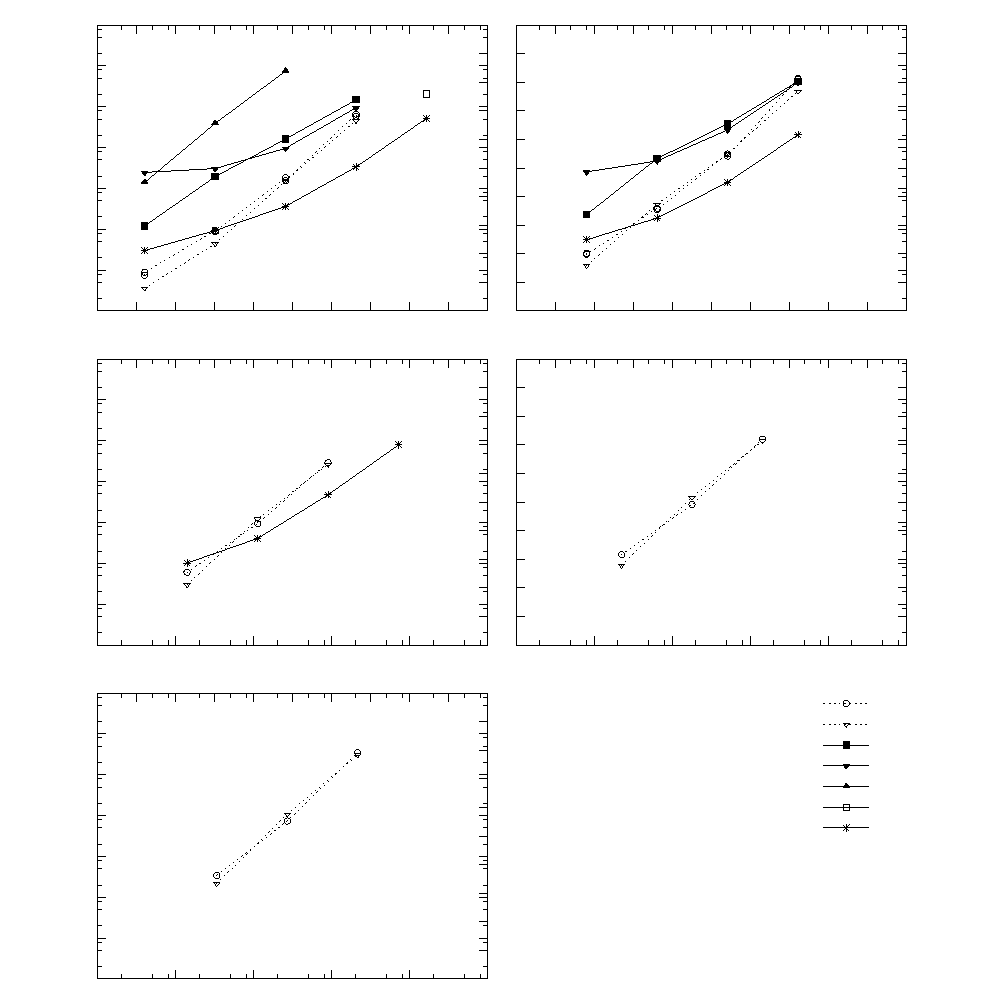
\includegraphics{ConstCoeffPoissonScaling}}%
    \gplfronttext
  \end{picture}%
\endgroup
